%!TEX ROOT=main.tex

\section{Software architecture}\label{sec:software-architecture}

\begin{figure}[h!]
    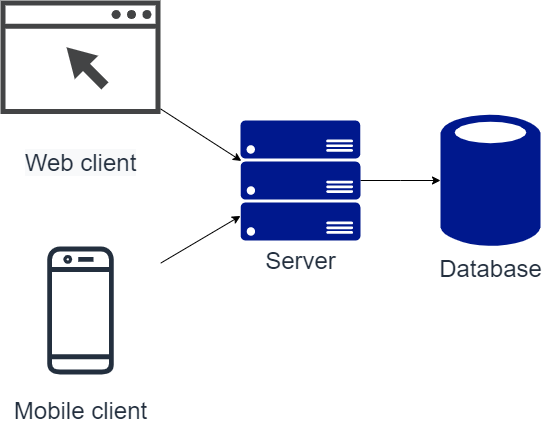
\includegraphics[width=0.75\textwidth]{images/high-level-architecture}
    \caption{High-level software architecture}
    \label{fig:high-level-architecture}
\end{figure}

Software architecture has been proposed with scalability and multiple types of client applications in mind.
As shown in figure~\ref{fig:high-level-architecture}, server is a standalone application separated from client applications.
Such separation allows sharing business logic across different client applications without a need of rewrite.
Another benefit is the simplicity of scaling.
New instance of the server application might be deployed behind load balancer as needed.

More specifically application is built using Model-View-Controller (MVC) architecture.\cite{wiki-mvc}
View component in MVC is a representational layer.
User interacts with the application through mentioned layer.
In case of this application View component is represented by client applications.
Model component represents business logic and Controller serves to bind View and Model.
Model and Controller components are encapsulated in server part of this application.

\begin{figure}[h!]
    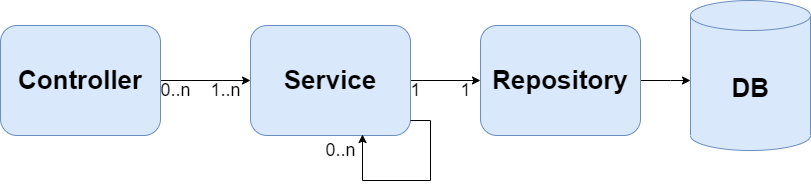
\includegraphics[width=1\textwidth]{images/server-mvc-spring}
    \caption{High-level software architecture}
    \label{fig:server-mvc-spring}
\end{figure}

Detailed server architecture displayed in figure~\ref{fig:server-mvc-spring}.
Repository serves as a Data Access Object (DAO).
Each DAO defines the set of allowed operations over a specific entity of the domain model.
Service is an implementation of business logic.
Each Service has exactly one related Repository.
Other entities Repositories should be accessed via their Service component, hence 0-to-n cardinality from Service to Service.
Complex business logic scenarios with several Service components calls might be encapsulated using the facade design pattern.
Controller creates API endpoint mapping, e.g.\ in www.domain.com/users '/users' is an endpoint mapping.

Described architecture is supported out of the box by major web development frameworks as Spring (Java/Kotlin), Django (Python), Rails (Ruby).\cite{spring,django,ruby} etc.
This, alongside with preservation of the single-responsibility principle~\cite{wiki-srp} enforced by the idea of MVC, allows for rapid development of maintainable applications.